% !TEX root = ../report.tex

\chapter{Software}\label{software}
The software architecture was centred on the event-driven implicit implication
architectural style~\cite{garlan1993introduction}. With regards to software architecture, this means
modules are signalled to start by other modules and this is propagated through
the system with events cascading to trigger other actions within the system.

To implement this architecture, each part of the system can be defined as its own
module with a function which triggers its invocation and a function which can
broadcast events if required. One possible implementation of this system uses
the publish--subscribe model. Nodes may publish data on communication channels
referred to as topics, which triggers all nodes which have subscribed to the
topic to take some responding action. This pattern has the advantage that
the resulting software has strong support for reuse, as new architecture
components can be dynamically added at runtime by subscribing to the appropriate
topics. Loose coupling between modules means that maintenance and testing
of each module can take place independently and significant changes to the
system can also be made without the need for major architectural modifications.

In robotic systems, this data-oriented approach is highly beneficial as each of
the sensor
and actuator systems can run independently without requiring knowledge of
implementation details of other parts of the system. This
reduces the risk of system crashes, as module crashes are isolated, increasing
robustness.

A true implementation of the event-driven implicit invocation style would have all
actions being taken only in the callback responses, with modules being inactive
the rest of the time. However, in a dynamic environment such as a robot with many
topics being published many times per second, it is inefficient and unsafe to have
large amounts of code in the callback functions, which block other operations from
taking place. It is therefore often beneficial for nodes to have a polling loop
in which they handle computationally expensive functionality, with
callbacks only setting up the data required by this loop.

\section{ROS}\label{soft/ROS}
In order to implement this architecture, and following extensive research
(c.f.\ Section~\ref{litreview/ROS}), the Robot Operating System (ROS) was
selected as a platform. The ROS framework makes it simple to design and implement
individual modules as nodes, and uses a central \verb|roscore| control
node to manage interactions between nodes, which communicate by publishing and
subscribing to topics.

\subsection{Design}\label{soft/ROS/design}
Following the decision to use ROS to implement our chosen architecture, a modular
approach was adopted for the design of each of the components within the system.
Figure~\ref{fig:software_block_diagram} shows a system-level block diagram visualising the
primary channels of data flow between modules. This structure allows a
data-driven approach to module development, making individual modules easily
interchangeable due to the high level of decoupling. Sensors, actuators and
control nodes can therefore easily be changed at a later date without requiring
major changes to the overall software structure.

\begin{figure}[!ht]
	\centering
	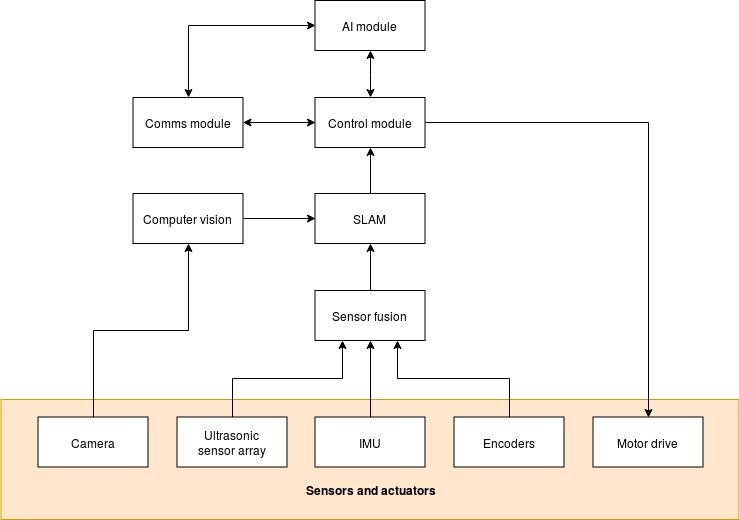
\includegraphics[width=1\textwidth]{diagrams/software_diagram.png}
	\caption{High-level software block diagram}\label{fig:software_block_diagram}
\end{figure}

ROS provides two client libraries, \verb|rospy| and \verb|roscpp|, which allow
programming nodes in Python and C++, respectively. Although the majority of
the system will be programmed in Python, the choice of programming languages
means that timing or processing-sensitive operations can be written in a
lower-level programming language as required.

Individual nodes can be started from the command line using the \verb|rosrun|
tool, or can be included in ROS launch files, which allow multiple nodes to
be run simultaneously with any number of parameters. Launch files, which are
written in a ROS-specific XML format, enable the
creation of multiple configurations of nodes with different parameters,
allowing different system setups to be tested easily. Launch files can be run
using the \verb|roslaunch package_name file.launch| command.

ROS nodes are created by scripts within ROS packages, which are located in a
Catkin workspace. Catkin, a CMake-based build system used to build ROS
packages~\cite{gitcatkin}, requires a strict directory structure, with each
package containing \verb|launch|, \verb|script| and \verb|msg| directories
containing launch files, node scripts, and message type definitions,
respectively.

\subsection{Implementation}\label{soft/ROS/impl}
In order to enable rapid development of the system, ROS packages were
primarily written in Python. Four packages specific to the project were
created:

\begin{itemize}
	\item \verb|crues_sensors| for hardware interfaces with sensors and nodes used
	for processing sensor data and camera imagery
	\item \verb|crues_actuators| for hardware interfaces with actuators
	\item \verb|crues_comms| for nodes handling communication between robots
	\item \verb|crues_control| for control nodes and AI modules, as well as
	system-level launch and configuration files
\end{itemize}

In addition, a number of third-party packages were installed to aid with
sensor fusion, mapping, and other specific tasks.

Each of the individual modules shown in \ref{fig:software_block_diagram} was
implemented as a ROS node, generally encapsulated in a single Python
script. In order to adhere to best practices and ensure consistency across
the code base, each node was represented as class, with an
\verb|__init__()| method initialising the node and a \verb|spin()| method
which is called to run the node's main loop. In nodes which perform
recurring work, such as polling sensors for data, this method uses a
\verb|rospy.Rate| object to schedule tasks, whereas nodes that respond to
events on subscribed topics simply call \verb|rospy.spin()|, which
prevents the script from exiting until a ROS shutdown signal is received.

The \verb|rospy.Publisher| class is used to publish messages of a
pre-determined type to a topic with a given name. Similarly,
\verb|rospy.Subscriber| is used by nodes wishing to listen for messages on
a specific topic. The constructor of this class specifies a callback
function, which receives the message as an argument. By loading parameterised
values at startup, the code maintains flexibility, as different values can
be used in launch files for different applications.

Listing~\ref{lst:ros_node} shows an example of a ROS node that publishes
at a predefined rate. The rate can be passed to the node as a parameter in
the launch file, and in this case defaults to \SI{10}{\Hz}. The data is
set by a callback method, which is called by a subscriber to another
topic. In general, callback methods were kept very short in order to
prevent blocking of the subscriber's thread, with any processor-intensive
work executed in the main loop. In this case, the node simply publishes the
data received on the subscribed topic unaltered.

\begin{lstlisting}[caption={Example ROS node}, label={lst:ros_node}]
#!/usr/bin/env python
import rospy
from std_msgs.msg import String


class Echo:
    def __init__(self):
        rospy.init_node('node_name')
        self.data = ""
        rospy.Subscriber('input_topic', String, self._callback)
        self.pub = rospy.Publisher('echo_topic', String, queue_size=10)
        self.rate = rospy.Rate(rospy.get_param("~rate", 10))

    def spin(self):
        while not rospy.is_shutdown():
            self.pub.publish(self.data)
            self.rate.sleep()

    def _callback(self, msg):
        self.data = msg.data


if __name__ == '__main__':
    try:
        node = Echo()
        node.spin()
    except rospy.ROSInterruptException:
        pass
\end{lstlisting}

\subsection{Software versions}
Various third-party software packages were used throughout this project.
Below are details and rationale for the choices of software used
widely throughout the system; additional packages used for specific modules
are detailed in the following sections that concern the respective modules.

\subsubsection{Operating system}
The Raspberry Pi 3 B+ allows the installation of a number of Linux-based
operating systems, of which Raspbian, a derivative of Debian, is the
recommended default operating system. Initially Raspbian Stretch was chosen;
however, problems were experienced with slow performance and heavy CPU usage.
Research suggested that, while ROS officially supports Debian-based
systems, performance is significantly optimised in ROS distributions for
Ubuntu. For this reason, it was decided to switch to Lubuntu 16.04, a light-weight
distribution based on Ubuntu with the LXDE desktop environment.
In order to minimise overhead, the desktop environment was disabled. The
operating system was installed from an image produced by Ubiquity
Robotics (available for download from
\url{https://downloads.ubiquityrobotics.com/pi.html}), which is
bundled with various robotics tools, including an installation of ROS
Kinetic.

\subsubsection{ROS}
The selected ROS distribution, ROS Kinetic Kame, was released in 2016. The
decision to use this version over more recent releases such as the 2018
Melodic Morenia release was informed by the wide availability of packages
for the former distribution, some of which are yet to be released on more
recent platforms.

\subsubsection{Python}
This project currently uses Python 2.7, which will no longer be supported
after January 2020~\cite{python2-eol}. The reason for this choice was the
lack of official support for Python 3.x in ROS Kinetic. While in principle
it is possible to use Python 3 with ROS, various compatibility issues may
arise~\cite{medium-ros-python3}. In the interest of stability,
it was decided to use the older version. Migration to ROS 2, which is
currently under heavy development but will have native support for Python
3, is recommended in future~\cite{ros2}.

\subsubsection{RPi.GPIO}
For hardware interactions with the Raspberry Pi's GPIO pins, RPi.GPIO and
WiringPi were considered. RPi.GPIO was selected as it is widely adopted in
the Raspberry Pi community, and is used as the basis for a number of other
GPIO libraries, such as GPIO Zero. Over the course of the project, various difficulties were encountered with
the library, including problems with the edge-detection implementation which
resulted in frequent ultrasonic sensor timeouts, and the lack of a hardware
PWM interface. Migration to WiringPi, which does not suffer from these problems
is suggested in future.


\subsection{Testing}\label{soft/ROS/test}
ROS provides a number of packages for testing and debugging systems. These
include \verb|rviz|, which generates spacial visualisations of data published
on specific topics, \verb|rqt_plot|, which allows real-time graphing of
numerical data, and \verb|rqt_graph|, which displays ROS computation graphs
illustrating interactions between nodes. Each of these packages were used
extensively in testing both individual nodes and system architectures.
Figure~\ref{fig:rqt_graph} shows the computation graph of the overall system,
generated by \verb|rqt_grpah|, with nodes represented by ellipses and topics
shown as rectangles.

In addition to these tools, which were mainly employed on code running on the
RPis, a suite of unit tests was written to prevent regressions. In
order to allow these tests to run on desktop PCs before deploying to the
RPi, the Python \verb|unittest.mock| mocking framework was used to
replace ROS functionality that would otherwise require a ROS master node to
be running. In addition, a mock version of RPi.GPIO was written in order to
allow simulation of hardware interactions in tests. This took the form of a
\verb|GPIO_MOCK| Python module, with functions and classes mirroring those in
RPi.GPIO. Listing~\ref{lst:gpio_import} shows how to ensure that the correct
library is imported depending on the platform the code is running on. This
takes advantage of the fact that RPi.GPIO only runs on Raspberry Pis and cannot
be installed on desktop computers.

\begin{lstlisting}[caption={Import statement for RPi.GPIO library}, label={lst:gpio_import}]
try:
    import RPi.GPIO as GPIO
except ImportError:
    from crues_tools import GPIO_MOCK as GPIO
\end{lstlisting}

\begin{landscape} % Rotates the image on the page
\global\pdfpageattr\expandafter{\the\pdfpageattr/Rotate 90} % Rotates the page in the PDF output
\begin{figure}[!p]\centering
    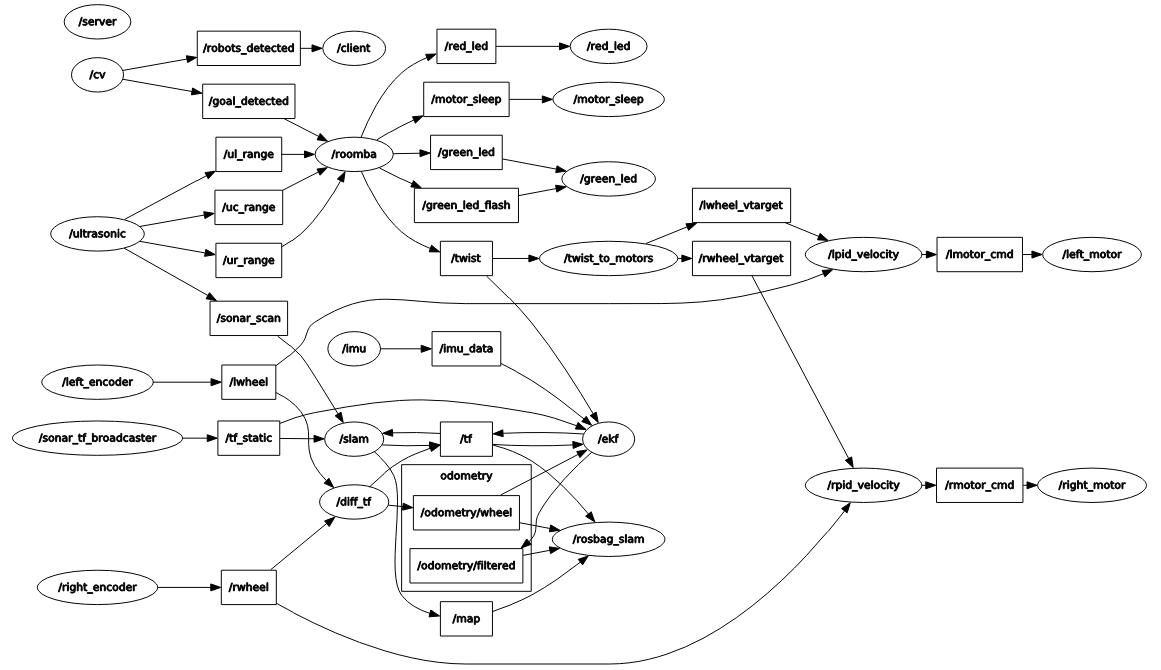
\includegraphics[width=1\linewidth]{graphs/rqt_graph}
    \caption{ROS computation diagram showing interactions of nodes and topics for overals system}\label{fig:rqt_graph}
\end{figure}
\end{landscape}
\global\pdfpageattr\expandafter{\the\pdfpageattr/Rotate 0}


\subsection{Deployment}\label{soft/ROS/deploy}
Since system testing was closely tied to the hardware of the robot, the
ability to rapidly deploy changes to the robot was crucial to the
development process. To this end, a shell script (\verb|deploy.sh|) was
written to copy any changes to robots connected to the network. The script
uses \verb|rsync| to copy any modified source or configuration files in
the Catkin workspace, and fetches any output files generated by previous
executions of the code. Since the RPis are unable to retain
system time between boot cycles, and \verb|rsync| relies on system time to
detect file modifications, the script additionally synchronises the system time
of the Pi to the host machine. The system time is set using UTC in order
to prevent problems caused by time zones and daylight saving time.

The installation of software dependencies proved to be less trivial due to
difficulties connecting to the internet and WANET simultaneously.
Dependencies were initially installed manually on a single Pi connected to
the internet, and were then transferred to the other robots by copying an
image of the SD card. This method had the additional benefit of ensuring
that all Pis were running the same versions of any dependencies.

\section{Communication}\label{soft/comms}
The communication node's requirements were to allow the robots to
be able to send and receive messages to each other. The structure
of these messages should allow for any object to be able to be sent
regardless of the data types, depth or complexity of the objects.
Each robot should also be able to simultaneously listen for
incoming messages whilst sending messages to a different robot.
With the aim of allowing scalability, the communication system
should be able to handle robots listening to multiple robots at the
same time, whilst also being connected to send messages to different
robots.

The communication system also requires a network or communication
technology to allow all of the robots in the system to be able to
communicate with each other. Each of the robots will also require
a unique identifier to allow sending messages to specific robots
rather than broadcasting all messages to all robots.

\subsection{Design}\label{soft/comms/design}
In order to implement these requirements,	 the first decision was the
method the robots were going to use to communicate. A few options
for this were considered such as Bluetooth and WiFi. After
researching and considering these options, the decision was taken
to use a Wireless Ad-hoc Network (WANET).

WANET is a wireless network where the nodes can be located anywhere
globally and does not require any infrastructure such as a router. The underlying design is such that the nodes believe
they are part of a single-hop or multiple-hop wireless network at the
physical layer and the data link layer as part of the MAC sublayer~\cite{rajesh2015congestion}. The wireless channels are often shared
and use carrier sense multiple access protocols to handle multiple
nodes attempting to use the channel at the same time. This is known
as link-level congestion and increases packet service time,
decreasing utilization and overall throughput. Although scalability
is an important factor, it was deemed a WANET's handling of
congestion was sufficient given the anticipated level of
communication across the system at any time would be low.

Each node in the WANET is assigned a local IP address.
Anything that connects to the network can then send messages through
the network provided it knows this address. As a result, any given robot
needs a method of finding this address to send messages to other robots. The simplest method for this is to use a lookup table
that maps the robot's name to their fixed IP in the network, allowing
all nodes in the network access to this.

After deciding to use WANET, a decision  had to be made in how to format
the data to send over the network. A few options were available such as
using JSON, XML or a custom-structure. It was decided the best option was
to use JavaScript Object Notation (JSON) objects after consultation with
Dr~Irvine as discussed in Section~\ref{pm/consultations}. JSON is a
standard data-interchange format that is easy for humans to read and write
as it uses attribute-value pairs and array data types.

After considering various options for the structure of the communication process,
a client-server system was decided upon. The client is the node
responsible for sending the messages whilst the server is responsible
for listening for incoming messages. As these are separate nodes,
they will work independently of each other and will allow the
robot to send and receive messages simultaneously.

\subsection{Initial Implementation}\label{soft/comms/iniimpl}
To implement these requirements a \verb|comms.py| file was created which contained
the function definitions and address lookup table that the server and
client nodes would use to communicate. Firstly, a Python dictionary of the
robot's IP addresses and a laptop's IP address for testing purposes was created.
A \verb|lookupIP(name)| function and a \verb|lookupname(ip)| function were created for
modularity and maintainability. Secondly, functions were required that could
create the JSON message (\verb|tojson()|) and extract the data from
the message (\verb|fromjson()|).

\begin{lstlisting}[caption={JSON Conversion Functions}, label={lst:comms_json}]

def tojson(host_ip, hostname, data):
    # receiver ip and hostname, our ip and hostname, classname
    sender_ip = socket.gethostbyname(socket.gethostname())
    header = [host_ip, hostname, sender_ip,
    Address_lookup.lookupname(sender_ip), type(data).__name__]
    content = [header, data]
    message = json.dump(content, separators=(',', ':'))
    return message

def fromjson(packet):
    message = json.loads(packet)
    try:
        target = message[0][0]
        if target == socket.gethostbyname(socket.gethostname()):
            return message[1]
        else:
            return -1
    except IndexError:
        return -2
\end{lstlisting}

The header created includes the IP and name of both the sender and the
receiver as well as the type of Python object which the data is. The header
and the data to be sent are converted to JSON and returned as a single
string. When converting from JSON, the receiver checks that it was the
intended recipient of the message, returning $-1$ if it was not, before
returning the data object located at index 1 (header is index 0). These
are the four helper methods used by the \verb|send()| and \verb|listen()|
methods.

In order to physically send and receive the data the Python Socket library
is used~\cite{socketServerDocs}. This interface's \verb|socket()| function
returns a Socket object whose methods implement the Unix socket system calls.

\begin{lstlisting}[caption={send() Function}, label={lst:comms_send}]
# data is python object to send
def send(hostname, data):
    host_ip = lookupip(hostname) # The remote host
    port_number = 8001 # The same port as used by the server
    message = tojson(host_ip, hostname, data)
    s = socket.socket(socket.AF_INET, socket.SOCK_STREAM)
    if not s.connect_ex((host_ip, port_number)):
        s.sendall(message) # Sends string (of JSON)
        s.close()
\end{lstlisting}

Listing~\ref{lst:comms_send} shows the \verb|send()| function, which looks up the IP of the destination and gets the JSON
object of the message. It then attempts to connect using the \verb|connect_ex()|
which returns 0 if successful. If so, it can then use the Socket methods to send
the data and then close the connection.

When listening for incoming messages, the created Socket object must bind to
an IP address and port number. The address \verb|0.0.0.0| allows the node to listen
to any incoming messages. Listing~\ref{lst:comms_listen} shows the \verb|listen()| function which starts the node listening
whilst setting the number of queued connections allowed (set here to 2 but can
be increased when scaling the system to use more agents). Once the socket
accepts a connection, packets received can continually be stored
until no more data is received, after which the connection can be closed and
the data read from the JSON strings and returned.

\begin{lstlisting}[caption={\texttt{listen()} function}, label={lst:comms_listen}]
def listen():
    PORT = 8001 # Arbitrary non-privileged port
    s = socket.socket(socket.AF_INET, socket.SOCK_STREAM)
    s.bind(('0.0.0.0', PORT))
    s.listen(2)
    conn, addr = s.accept()
    packets = ''
    while 1:
        packet = conn.recv(1024)
        if not packet:
            break
        packets += packet
    conn.close()
    message = fromjson(packets)
    return message
\end{lstlisting}

\subsection{Initial Testing}\label{soft/comms/initest}
This implementation was set up and initially tested between a laptop and a
RPi by remotely connecting to the RPi. When this succeeded in sending
multiple messages between each device, a further RPi was remotely connected to and
an attempt was made to send messages between RPis. Again this was successful,
demonstrating the basic functionality of the communication system.

During more extensive testing, an important issue with the previous
code was found. When nodes were sending messages to each other simultaneously
at least one of the nodes would fail. For example, if robot A sends a message to
robot B but before the message has finished sending, robot B sends a message to
robot A; then the receiver of robot B crashes and robot A never receives the message.
If robot B were to send to a third robot, C, then robot B's receiver would still
fail as would one of either robot B or C.

As a result of this bug, the implementation had to be changed to handle
multiple connections properly. Various potential solutions were discussed,
such as using multiple ports --- so as not to kill the socket connection when
attempting to connect again --- or to use a multi-connection selector as part of
the server to handle multiple requests \cite{multiconnectionServer}.
Alternatively, if the server can always be listening for incoming messages by
utilising multiple threads then there would be no system downtime and
thus, each message would be successfully sent. As a result, a multi-threaded version
of the existing code was implemented.


\subsection{Multi-Threaded Implementation}\label{soft/comms/mtimpl}

A multi-threaded implementation was created by defining two classes, namely: \verb|ThreadedTCPServer| and
\verb|ThreadedTCPRequestHandler|, to be used by the listener as shown in
SocketServer documentation~\cite{socketServerDocs}.

\begin{lstlisting}[caption={ThreadedTCPRequestHandler}, label={lst:comms_tcprequest}]
class ThreadedTCPRequestHandler(SocketServer.BaseRequestHandler):
    def messageHandler(self, x):
        print x

    def handle(self):
        data = self.request.recv(1024)
        message = fromjson(data)
        self.messageHandler(message)

class ThreadedTCPServer(SocketServer.ThreadingMixIn, SocketServer.TCPServer):
    pass
\end{lstlisting}

The \verb|listen()| function was changed to take in a handler parameter. This was
passed a function which is used instead of the \verb|messageHandler()| function in
the \verb|ThreadedTCPRequetHandler| before it is used to create a \verb|ThreadedTCPServer|
object as shown in Listing~\ref{lst:comms_listen2}.

\begin{lstlisting}[caption={listen() Function 2.0}, label={lst:comms_listen2}]
def listen(handler):
    ThreadedTCPRequestHandler.messageHandler = handler
    HOST, PORT = "0.0.0.0", 8001
    server = ThreadedTCPServer((HOST, PORT), ThreadedTCPRequestHandler)
    ip, port = server.server_address
    # Start a thread with the server -- that thread will then start one
    # more thread for each request
    server_thread = threading.Thread(target=server.serve_forever)
    # Exit the server thread when the main thread terminates
    server_thread.daemon = True
    server_thread.start()
    return server
\end{lstlisting}

The \verb|handler| object passed is a function that will publish the message contents so
relevant subscribers can use the data received from the other robot. As a new
thread is being created for each request, node crashes from interruptions no longer occur.

\subsection{Multi-Threaded Testing}\label{soft/comms/mttest}
In order to test this version, it was important to first ensure that the
previously successful tests remained successful. Therefore,
the same initial tests were applied to this implementation and were
successful as expected. To test whether the new implementation was
thread-safe, a number of tests were executed.

The first test involved creating a loop that would send 100 messages from robot
A to robot B. When this succeeded without any node crashes, the test was repeated
but with robot B sending messages to robot A at the same time. This test would
have previously crashed each of the robot's nodes but, with each new connection
request handled in a different thread, the test was successful. The test was then
repeated once more with robot B sending messages to robot C instead of robot A,
again resulting in a successful test with no messages lost.

Finally, a stress test was carried out. The previous test was executed again with
the limit on the number of messages being sent removed, and so the node would,
in theory, continue to create new threads to listen to the incoming messages.
Initially, this worked, however, due to there being no delay between sent messages,
thousands of threads were created rapidly. This resulted in the node
crashing as the thread limit had been reached, however, this happened after over
50,000 messages. As a result, this was determined to be the upper limit of the system,
which is excessive for both this project's, and any reasonable purposes, hence, it was
determined that the system was sufficiently thread-safe to be used.

\section{PID Controller}\label{soft/PID}
A PID controller was used for each wheel to ensure a constant output
velocity at the target specified by the control node. The PID controller is
a feedback loop designed to eliminate errors in the actuator systems, ensuring
that the motors correct for any outside forces such as friction that act on the
motor. By tuning the gain terms $K_p$, $K_i$ and $K_d$ for the system in
question, a target velocity can quickly be approached without overshooting.

\subsection{Design}\label{soft/PID/design}
The PID control node from the ROS \verb|differential_drive| package was
used~\cite{diffdrivelib}. The node subscribes to a \verb|/wheel_vtarget| topic
which sets the target velocity of a wheel and a \verb|/wheel| topic which provides
the actual current speed of the wheel as determined by the encoders, and publishes
a command value to \verb|/motor_cmd|, which is subscribed to by the corresponding
motor drive node. The command is a signed float which is used by the drive node
to determine direction and PWM values. Listing~\ref{lst:pid_launch} shows the
XML used to create PID nodes for the left and right wheels. The parameters
\verb|pid/Kp|, \verb|pid/Ki| and \verb|pid/Kd| are specified in the CRUES
configuration file (\verb|crues_control/config/params.yaml|). The publishing rate
of the PID nodes was set to the rate of the encoders to avoid unnecessary
computation.

\begin{lstlisting}[caption={PID nodes in ROS launch file}, label={lst:pid_launch}, style=xml]
<node name="lpid_velocity" pkg="differential_drive" type="pid_velocity.py">
    <param name="out_min" type="double" value="-0.5" />
    <param name="out_max" type="double" value="0.5" />
    <param name="rolling_pts" type="int" value="2" />
    <remap from="~Kp" to="pid/Kp" />
    <remap from="~Ki" to="pid/Ki" />
    <remap from="~Kd" to="pid/Kd" />
    <remap from="~rate" to="encoder/rate" />
    <remap from="/wheel" to="/lwheel" />
    <remap from="/motor_cmd" to="/lmotor_cmd" />
    <remap from="/wheel_vtarget" to="/lwheel_vtarget" />
    <remap from="/wheel_vel" to="/lwheel_vel" />
</node>

<node name="rpid_velocity" pkg="differential_drive" type="pid_velocity.py">
    <param name="out_min" type="double" value="-0.5" />
    <param name="out_max" type="double" value="0.5" />
    <param name="rolling_pts" type="int" value="2" />
    <remap from="~Kp" to="pid/Kp" />
    <remap from="~Ki" to="pid/Ki" />
    <remap from="~Kd" to="pid/Kd" />
    <remap from="~rate" to="encoder/rate" />
    <remap from="/wheel" to="/rwheel" />
    <remap from="/motor_cmd" to="/rmotor_cmd" />
    <remap from="/wheel_vtarget" to="/rwheel_vtarget" />
    <remap from="/wheel_vel" to="/rwheel_vel" />
</node>
\end{lstlisting}

In addition to the PID node, the library has a \verb|wheel-loopback|
simulator node, which simulates the movement of wheels. This node was used in
order to evaluate PID tuning methodologies ahead of the slower process of tuning
the actual values on the physical robot. The various methods discussed in Section~\ref{litreview/robotics/pid} were attempted and outcomes recorded.

\subsection{Ziegler-Nichols}\label{soft/PID/zn}
As most of the research carried out pointed towards the Ziegler-Nichols
method as being an effective way of tuning PID, this was first tried directly
on the robot. In order to tune the PID in real time, the values of $ K_p
$, $ K_i $ and $ K_d $ were published to the ROS system from a terminal
while \verb|roscore| was running. $K_p$ was increased until oscillations were
seen in the system --- the determination of an oscillation was vaguely
defined across literature and hence this was done by eye --- and this was
set as the critical gain $K_u$ of the system. The period of oscillation
$T_u$ was then measured. From these values, a tuning table~\cite{mccormack1998rule}
of tuning rules was used to calculate values for the gains. The results of this
process are shown in Table~\ref{zn_pid_tuning}.

\begin{table}[!ht]\centering
\caption{Ziegler-Nichols PID tuning
\label{zn_pid_tuning}}
    \begin{tabular}{cccccc}
        \toprule
        \thead{Method} & \thead{$K_u$} & \thead{$T_u$ [\si{\second}]} & \thead{$K_p$} & \thead{$K_i$} & \thead{$K_d$}\\
        \midrule
		ZN & 775 & 0.14 & 465 & 6642 & 8.13\\
		ZN & 800 & 0.14 & 480 & 6857 & 8.4\\
		NO-OV & 775 & 0.14 & 155 & 2214 & 7.49\\
		NO-OV & 800 & 0.14 & 160 & 2240 & 7.47\\
        \bottomrule
    \end{tabular}
\end{table}

In practice, these values were found to be inaccurate
and produce an uneven stop-start motion in the movement of the robot.
This was due to these methods providing an aggressive gain and overshoot
which resulted in the motors being run at high speed followed quickly by
low speed to average to the correct speed. Due to the high current drawn by
the motors when stopping and starting, this additionally had implications on
the power consumption of the robots, with batteries being drained rapidly.
The NO-OV tuning rules, which are intended to limit the amount of overshoot,
mitigated this effect slightly, but still did not result in accurate
velocities.


\subsection{Manual Tuning}\label{soft/PID/man}
Due to the problems outlined above, the library simulation was used to
find a usable tuning method. A more practical solution was
found~\cite{practicalPID}, which approached the problem without calculating
values. Using the simulation and output graphs obtained from the ROS
\verb|rqt_plot| package to determine correct behaviour, $K_p$ was
increased until the system oscillated with a constant amplitude.
$K_p$ was then halved and $K_i$
introduced to increase the rate of change in the system. $K_d$
could then be slowly increased to minimise the overshoot in the system.

Additional improvements were achieved by scaling the output of the PID loop
in the drive node. As the PWM values used by \verb|RPi.GPIO| are in the range
$[0; 100]$ and the velocities published to \verb|/wheel| are in \si{\metre\per\second}
(with a typical range of $[0; 0.5]$), high gain values are required to ensure
the output is on the correct order of magnitude. A scale factor and an offset
were therefore introduced in the motor drive node as shown in
Listing~\ref{lst:pid_scaling} in order to map inputs from an arbitrary
input range to the range $[-100; 100]$. Using $-0.5$ for \verb|~range_min| and $0.5$
for \verb|~range_max| resulted in the lower gain values shown in
Table~\ref{manual_pid_tuning}, and appeared to result in a slight reduction in
overshoot.

\begin{lstlisting}[caption={Output scale factor in drive node}, label={lst:pid_scaling}]
class Motor:
    def __init__(self):
        # ...
        self.range_min = rospy.get_param('~range_min', -1.0)
        self.range_max = rospy.get_param('~range_max', 1.0)
        self.scale_factor = 200.0 / (self.range_max - self.range_min)
        self.offset = (self.range_min + self.range_max) / 2
        # ...

    def _tick(self):
        # ...
        pwm_val = (self.cmd - self.offset) * self.scale_factor
        # ...
\end{lstlisting}

\begin{table}[!ht]\centering
\caption{Manual PID tuning results
\label{manual_pid_tuning}}
    \begin{tabular}{cccc}
        \toprule
        \thead{Method} & \thead{$K_p$} & \thead{$K_i$} & \thead{$K_d$}\\
        \midrule
        Before PID scaling & 102.5 & 2.5 & 0.88\\
        After PID scaling & 0.2775 & 0.0075 & 0.007\\
        \bottomrule
    \end{tabular}
\end{table}

\subsection{Rate control}\label{soft/PID/rate}

These values resulted in far less aggressive motion in the movement of the
robot. Despite this, velocity spikes still occurred, and following a
consultation with Dr Gordon Dobie (c.f.\ Section~\ref{pm/consultations}) a
rate control implementation was used.

Opposed to traditional PID, Rate Control employs only the $K_p$ and $K_d$ portions of
the equation and uses the current velocity as the base rate as opposed to 0~\cite{koditschek1987quadratic}. This allows the controller to maintain the speed
more smoothly and fewer spikes in motor current are required for the required
drive~\cite{kawamura1988local}. By removing the $K_i$ term, the speed will climb
more slowly from start-up and recover from dips in speed more slowly. This is
mitigated, however, by using the current speed as the base and therefore, a high
gain is not required to increase the speed to the required level.

Implementing this involved modifying the source
code for the \verb|differential_drive| package to add an adjustment term to the
previous output value. This eliminated the need for steady-state correction,
allowing $K_i$ to be set to $0$. Tuning the remaining values gave a proportional
gain $K_p = 0.176$ and a differential gain $K_d = 0.008$. This was tested and
resulted in significantly less aggressive motion of the robot and a increased
accuracy in output velocities.



\section{Odometry and Sensor Fusion}\label{soft/odometry}

\subsection{Wheel Odometry}\label{soft/odometry/wheel}

Wheel Odometry is derived in two parts. Firstly, as discussed in Section~\ref{soft/PID}, the velocity of each wheel is derived from the output of the
encoders. Then, with only these values and the distance between the wheels
(usually called the track of the wheels), the linear and angular velocities in two
dimensions can be derived. Furthermore, by tracking both of these values over
time, an estimate of global displacement can be attained. However, due to the lack
of reliability in the encoder data, this estimate is very likely to drift over
time.

\begin{figure}[!ht]
	\centering
	\includegraphics[width=0.75\textwidth]{diagrams/DiffDrive}
	\caption{The variables used to calculate wheel odometry}
	\label{fig:diff_drive_diagram}
\end{figure}

Let $u_l$, $u_r$ and $L$ be the velocities of the left and right wheels, and the
wheel track respectively, while $(x, y)$ and $\theta$ are the current displacement
and rotation from the origin. These values are reflected in Figure~\ref{fig:diff_drive_diagram}.

The ideal differential drive system has only two ``states'' of movement, either
moving in a straight line as a result of $u_l$ being equal to $u_r$ or rotating on
the spot as a result of $u_l$ being the inverse of $u_r$. This makes derivation of
equations for the odometry fairly simple.

When moving in a straight line, the linear velocity of the system is simply the
velocity of either wheel, in the direction $\theta$, while rotational velocity
should be $0$. To achieve the latter, the velocity used in the calculation is $0.5 (u_l + u_r)$, which is $0$ in the case where $u_l = -u_r$ and unchanged otherwise.
Splitting the velocities across the axes with the cosine and sine of $\theta$ achieves a reasonable result for these velocities.

Likewise, in the case of rotation, the linear velocities should be $0$. When the
robot rotates at some rate, say $\phi$, around its centre, the wheel must move at $u_r = 0.5 L \phi$ ($u_l = -u_r$ as the axis of rotation is the centre of the
robot). Like in the previous case, the velocity used in the calculation is to be 0
in the case where $u_l = u_r$, so the value
used is $0.5 (u_r - u_l)$, which is $0$ when the velocities are the same, and $u_r$ when they are opposite, preserving the direction of rotation.

The equations derived here are shown in Equations~\ref{eq:dotx} to~\ref{eq:dottheta}.


\begin{align}
\dot{x} & = \frac{(u_l + u_r)}{2} \cos(\theta) \label{eq:dotx} \\
\dot{y} & = \frac{(u_l + u_r)}{2} \sin(\theta) \label{eq:doty} \\
\dot{\theta} & = \frac{(u_r - u_l)}{L} \label{eq:dottheta}
\end{align}

\todo[inline]{This section needs to focus more on the differential\_drive package,
the various nodes it contains, inputs/outputs, etc. Formulas should
probably go in Background, as we did not implement these ourselves.}

\subsection{IMU}\label{soft/odometry/imu}

As was discussed in Section~\ref{elec/imu}, the IMU can also be used to
perform dead reckoning, and this can be fused with the wheel odometry to
improve the accuracy of the system.

For other nodes to use the IMU data, the readings had to be converted into
a ROS IMU message~\cite[sensor\_msgs/Imu.msg]{ROSDocs} consisting of: a ROS header message~\cite[std\_msgs/Header.msg]{ROSDocs};
a quaternion representing the orientation; a 3-element vector for
the rotational speed; a 3-element vector for the linear
acceleration; and covariance matrices for each of these measurements.
Listing~\ref{lst:imu_message} shows the the portion of \verb|imu_node.py| used to create IMU messages.


\begin{lstlisting}[caption={\texttt{\_publish\_data()} in \texttt{imu\_node.py}},label={lst:imu_message} , language=python]
def _publish_data(self):
    # ...
    msg = Imu()
    msg.header.frame_id = self.frame_id
    # Indicate orientation unknown:
    msg.orientation_covariance = [-1.0, 0.0, 0.0, 0.0, 0.0, 0.0, 0.0, 0.0, 0.0]
    msg.linear_acceleration = Vector3(acc[0], acc[1], acc[2])
    msg.angular_velocity = Vector3(gyro[0], gyro[1], gyro[2])
    # ...
\end{lstlisting}

There are a couple of points to notice in this excerpt. Firstly, the
covariance matrix for the orientation is set to a $-1$ followed by 0's.
This indicates that values for the orientation are unknown as we are only
using a 6-DOF IMU~\cite[sensor\_msgs/Imu.msg]{ROSDocs}. Secondly, the published values for the
x and y axes are negative the measured value. This is because, as
discussed in Section~\ref{elec/pcb}, the IMU had to be mounted at
\ang{180} relative to the robot frame (i.e. the x axis in the IMU faced
towards the back of the robot). While this would be possible to correct by
declaring a transform frame describing the IMU frame relative to the base
frame, this was thought to be a simpler solution. Because of this, the
frame in the header is set to \verb|base_link|.

The ROS spin functionality was used for the IMU, so
\verb|_publish_data()| is run at a set
frequency. This frequency, along with the topic the
IMU is published to, is set in the launch file, as
shown in Listing~\ref{lst:imu_launch}.

\begin{lstlisting}[caption={IMU node in ROS launch file}, label={lst:imu_launch}, style=xml]
<node name="imu" pkg="crues_sensors" type="imu_node.py">
    <remap from="~rate" to="imu/rate" />
</node>
\end{lstlisting}

\subsubsection{IMU Testing}\label{soft/odometry/imu/test}

To test the IMU integration with ROS, the ROS IMU visualisation software was used.
The robot was then rotated in each axis, and the output visualised.
Figure \ref{fig:imu_test} shows the IMU RVIZ visualisation along side the
corresponding position of the robot. Note that this only a small selection
of the test data, but all results appeared to accurately reflect the
movements performed.

\begin{figure}[!ht]
	\centering
	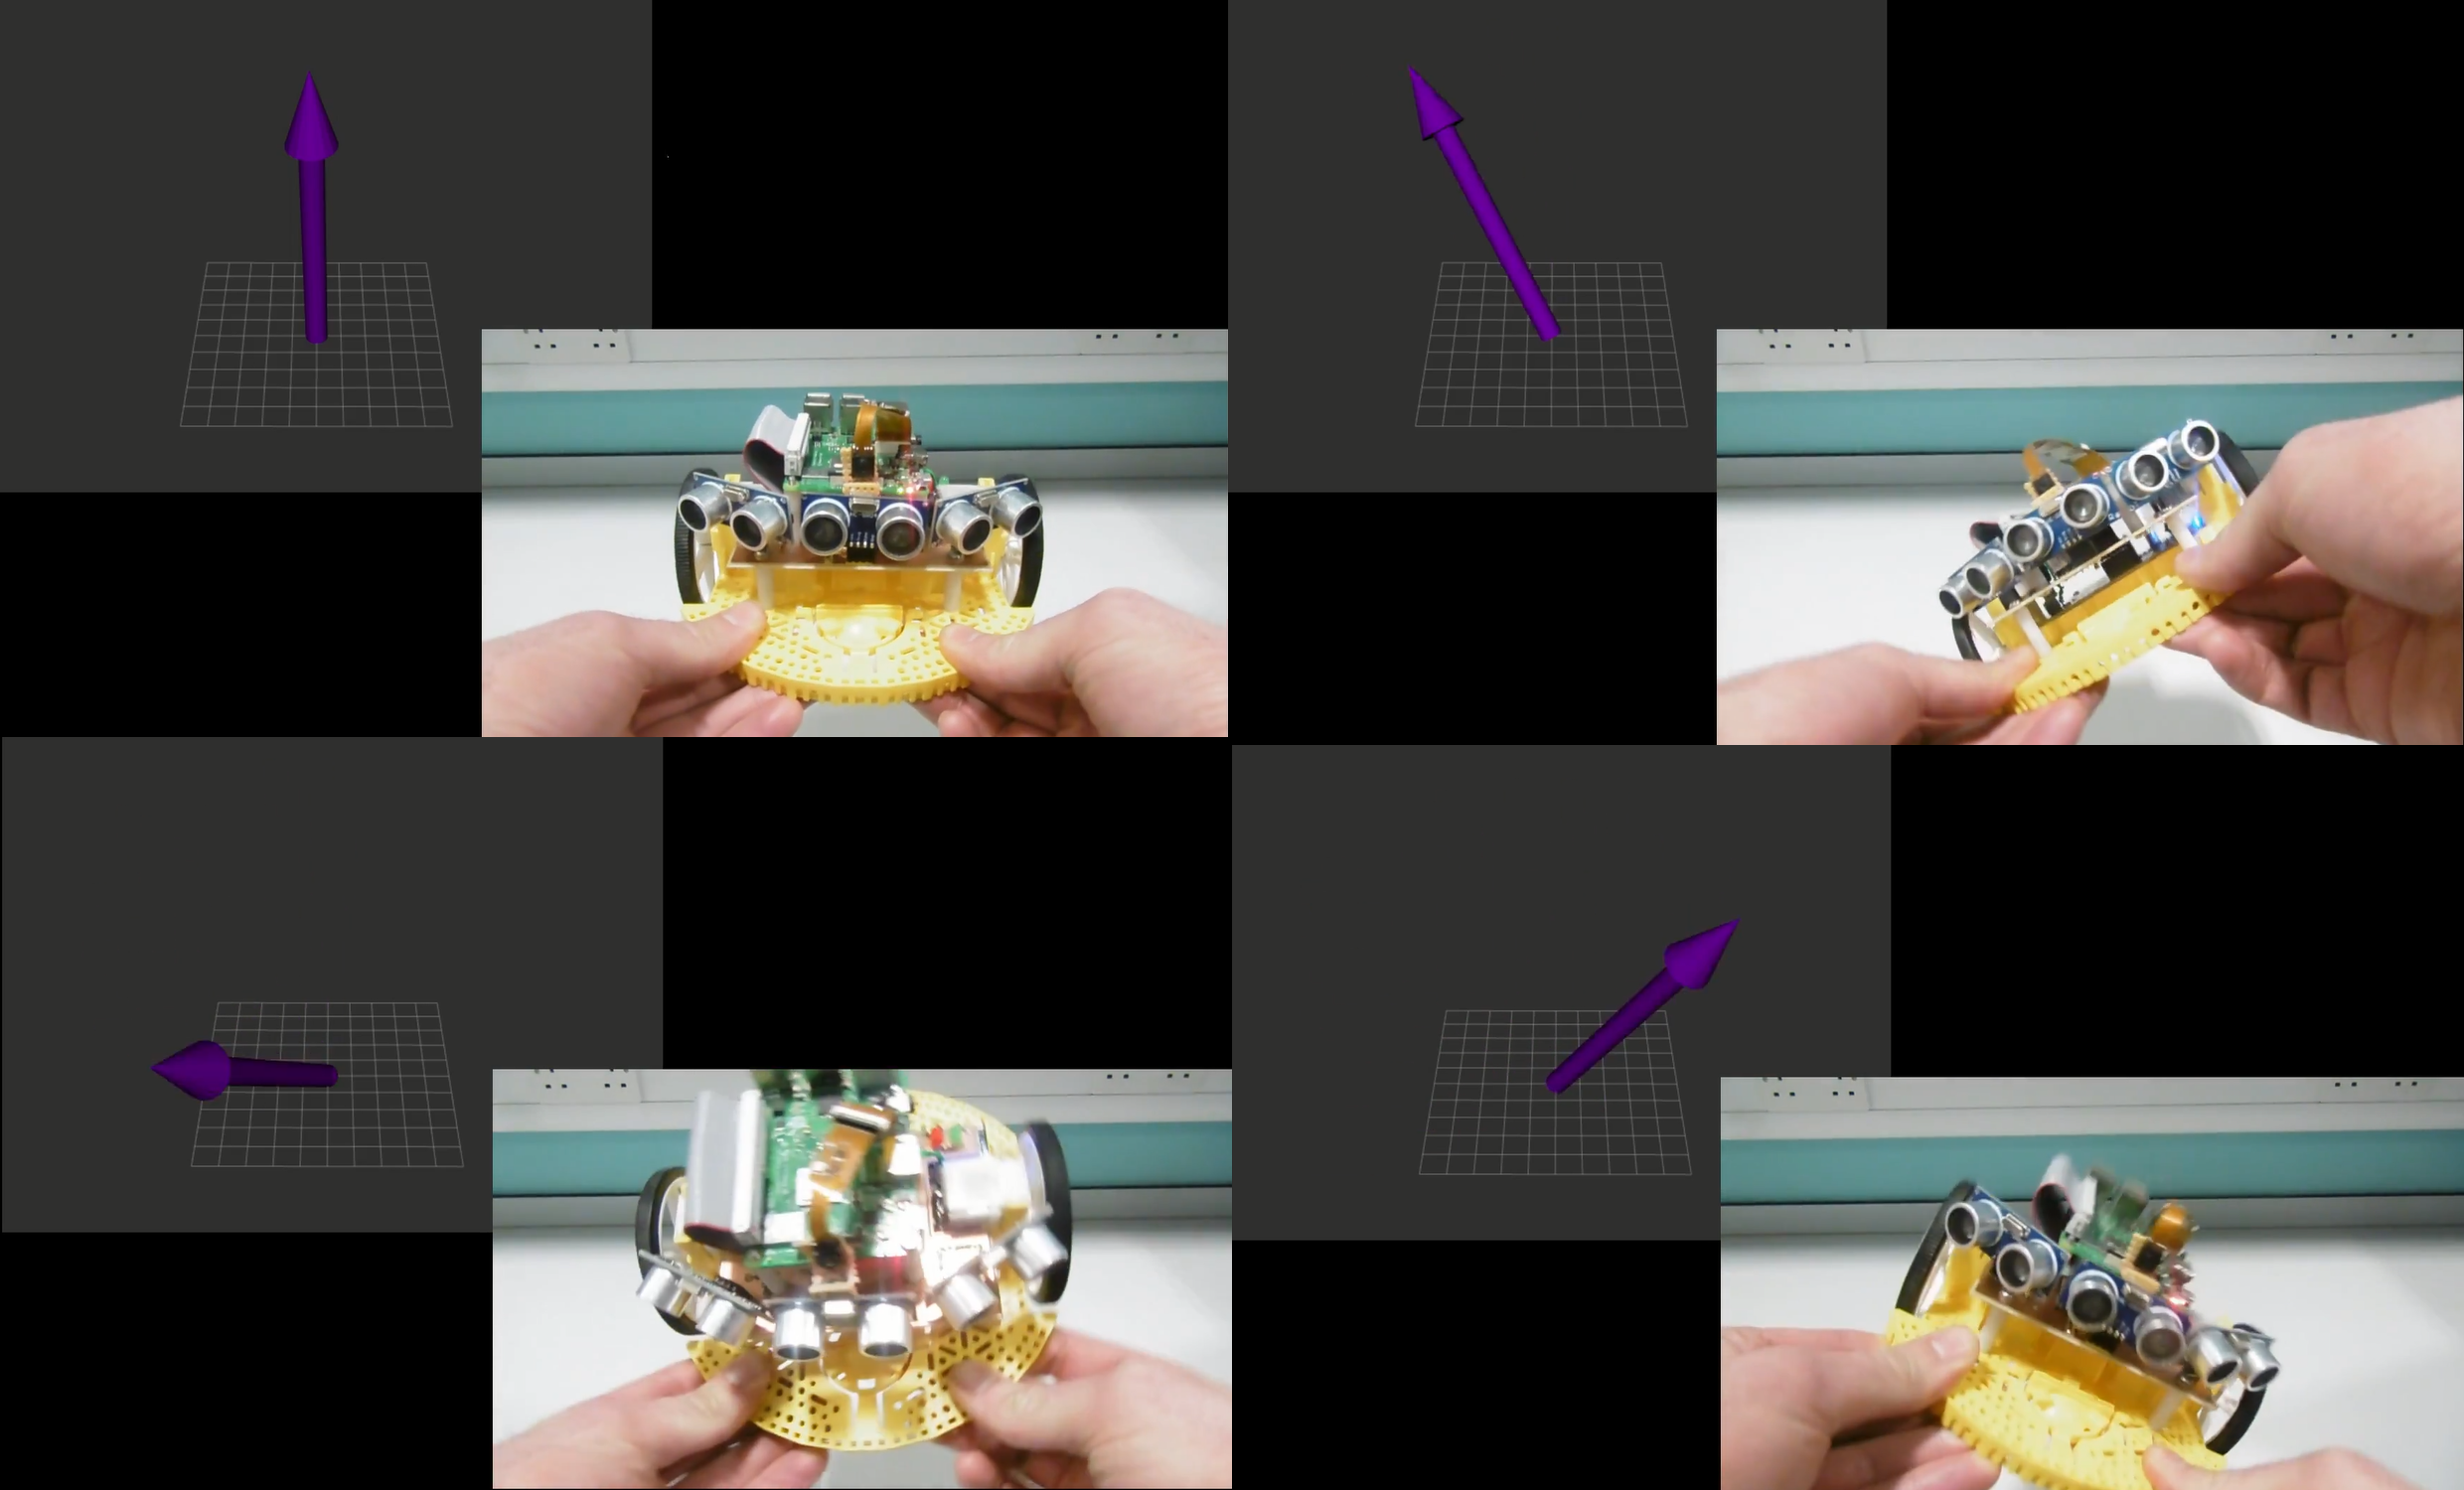
\includegraphics[width=1\textwidth]{IMUtest.png}
	\caption{IMU RVIZ test}\label{fig:imu_test}
\end{figure}

\subsection{EKF}\label{soft/odometry/ekf}

The ROS \verb|robot_localization| package~\cite{RosRobotLocalization} was used
to fuse the sensor data. This package contains implementations of
an EKF and a UKF (Unscented Kalman Filter). The latter has the advantage of higher
accuracy, particularly for highly non-linear transformations at the expense of
greater computational complexity~\cite{wan_unscented_2000}. In order to limit
computational overhead, the EKF implementation (\verb|ekf_localization_node|) was
chosen for use with this project. Listings~\ref{lst:ekf_launch} shows how an EKF
node is created in the main launch file.

\begin{lstlisting}[caption={EKF node in ROS launch file}, label={lst:ekf_launch}, style=xml]
<node name="ekf" pkg="robot_localization" type="ekf_localization_node"
      clear_params="true">
    <rosparam command="load" file="$(find crues_control)/config/ekf.yaml" />
    <remap from="/cmd_vel" to="/twist" />
</node>
\end{lstlisting}

The parameters used in the EKF are loaded from the \verb|ekf.yaml| file, which
specifies topics and configurations for each of the input sources. The
\verb|source_config| parameter for each source (i.e.\ wheel odometry and IMU data)
specifies which of the filter's 15 states the source updates. In the case of
odometry, the differential drive restrictions outlined in
Section~\ref{soft/odometry/wheel} mean that only the velocity in the $X$
direction relative to the robot's \verb|base_link| frame
and the yaw velocity (rotational velocity around the $Z$ axis) can be updated.
The IMU provides values for the yaw velocity and acceleration in the $X$ and
$Y$ directions.

\todo{Talk about graphics}


\begin{figure}[!ht]
  \centering
  \begin{subfigure}[b]{0.4\textwidth}
    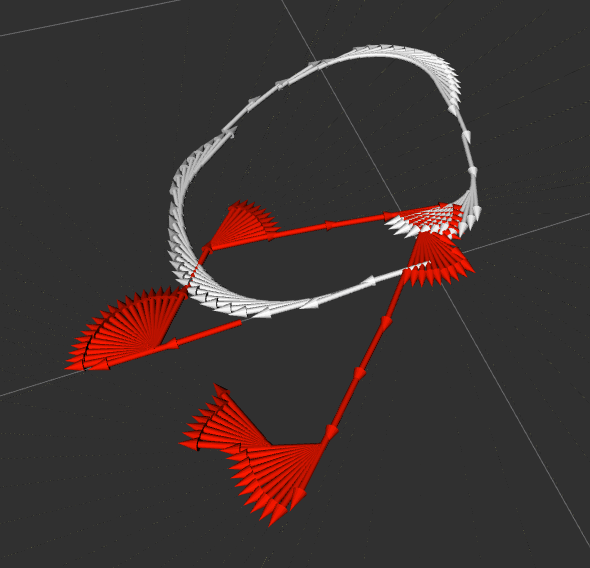
\includegraphics[width=\textwidth]{graphs/bad_ekf}
    \caption{Before optimising parameters}
    \label{fig:ekf_output/bad}
  \end{subfigure}
  ~
  \begin{subfigure}[b]{0.4\textwidth}
    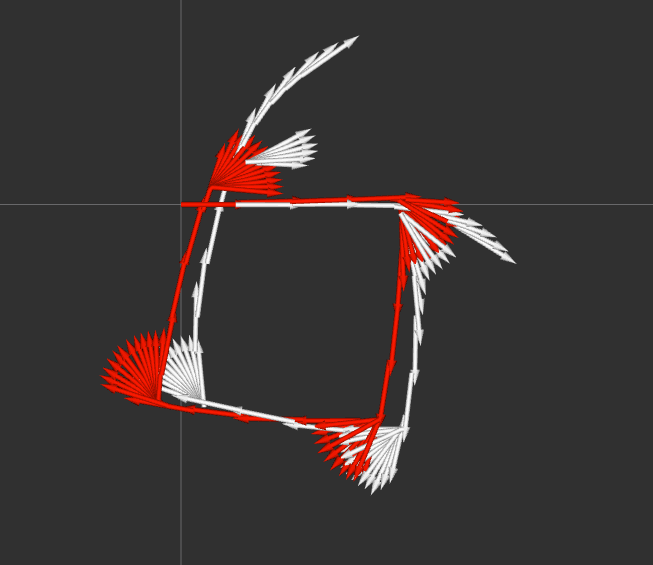
\includegraphics[width=\textwidth]{graphs/ekf}
    \caption{After optimising parameters}
    \label{fig:ekf_output/good}
  \end{subfigure}
  \caption[Odometry output]{Odometry output (wheel odometry in red, filtered odometry in white)}\label{fig:ekf_output}
\end{figure}



\begin{lstlisting}[caption={EKF YAML file}, label={lst:ekf_yaml}, style=yaml]
frequency: 50  # Frequency at which odometry is published in Hz
two_d_mode: true  # Ignore movement in three dimensions
publish_tf: true

odom0: odometry/wheel  # Topic on which wheel odometry is published
# Which values are provided by wheel odometry
# [x, y, z, roll, pitch, yaw, vx, vy, vz, vroll, vpitch, vyaw, ax, ay, az]
odom0_config: [false, false, false, false, false, false, true, false, false, false, false, true, false, false, false]
odom0_queue_size: 2
odom0_pose_rejection_threshold: 5
odom0_twist_rejection_threshold: 1

imu0: imu/data  # Topic on which IMU data is published
imu0_config: [false, false, false, false, false, false, false, false, false, false, false, true, true,  false, false]
imu0_queue_size: 5
imu0_pose_rejection_threshold: 0.8
imu0_twist_rejection_threshold: 0.8
imu0_linear_acceleration_rejection_threshold: 0.8
# True iff IMU returns acceleration without gravitational offset
imu0_remove_gravitational_acceleration: true

use_control: true
stamped_control: false
control_timeout: 0.2
# Which velocities are being controlled [vx, vy, vz, vroll, vpitch, vyaw]
control_config: [true, false, false, false, false, true]
\end{lstlisting}





\section{SLAM}\label{soft/SLAM}

As discussed in Section~\ref{litreview/slam}, Simultaneous Localisation and Mapping (SLAM) is an extensively 
researched and challenging topic. As a result of this, there are many existing implementations of a wide
variety of SLAM algorithms. The most commonly used package for this when working within the ROS framework
is \verb|gmapping|, an implementation of a particle filter, which is very well supported by the framework,
simply taking and producing standard ROS message types. It also provides a very rich suite of settings which
can be used to modify the functionality of the algorithm. The drawback of the package, and the wide variety
of settings available in particular, is the somewhat poor documentation it provides, which necessitated a
great deal of experimentation to achieve reasonable results, which will be discussed going forward.

\subsection{Package Overview}\label{soft/SLAM/package}

The \verb|gmapping| package takes in a \verb|LaserScan| message, as well as odometry data in the form of a
transformation frame (\verb|tf|). The odometry data is already produced by the sensor fusion module, so the
input parameter of \verb|gmapping| simply needs to be bound the same topic as the output of the EKF.

The scan data is more complex, as the package is intended for use with a LIDAR unit. The outputs of different
methods of active range finding are similar enough, however, that a rudimentary laser scan message could be
created simply by combining the three ultrasonic readings into a (admittedly fairly poor) approximation of a
LIDAR output. This will likely result in features in the map taking on rounded edges, as the wide range of
each sensor will allow it to find the walls of a corner earlier than the point.

The \verb|gampping| package, while providing some localisation via feature detection, and utilising the odometry
in creation of the map, does not actually perform true localisation. Another package, \verb|AMCL|, performs a
second iteration particle filtering algorithm on the map already processed by the mapping package, as well as
the scan data and odometry, and makes probabilistic approximations of the robot's location in the map. This is
mainly used to compensate for odometry drift, as mentioned in Section~\ref{soft/odometry/wheel}. A block diagram
indicating this relationship can be found in Figure~\ref{fig:amcl}.

\begin{figure}[H]
	\centering
	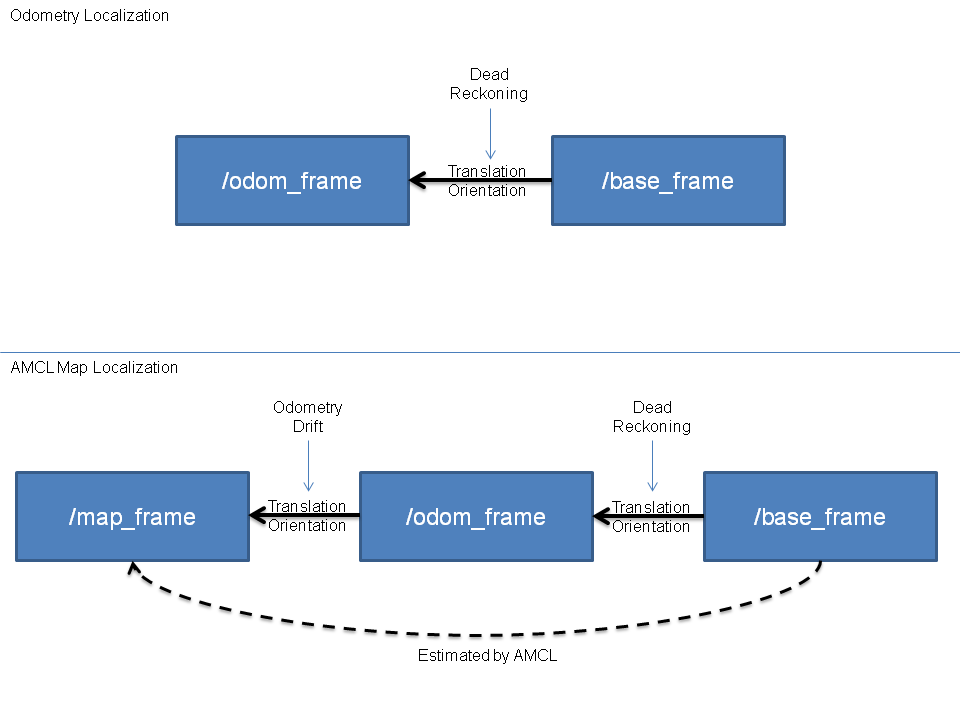
\includegraphics[width=\textwidth]{diagrams/amcl_localization}
	\caption{AMCL transform diagram~\cite{macenski_amcl}}\label{fig:amcl}
\end{figure}

Unfortunately, as particle filtering is an extremely taxing operation, it proved too taxing to run both
\verb|gmapping| and \verb|AMCL| at once on the RPi. Indeed, running only the mapping package proved problematic,
as certain configurations caused the entirety of the RPi's memory to be used, and led to some other ros packages
crashing as a result of being refused memory allocation. As a result of this, two parameters, ``particle'' and
``delta'' which respectively govern the number of steps in the filter and granularity of the generated map both
had to be reduced. Both of these will reduce the accuracy of the final output, but this appears to be an unavoidable problem.

\subsection{Tuning}\label{soft/SLAM/tuning}

The initial attempts at running \verb|gmapping| presented a number of problems immediately. For one, the map
generated was at entirely the wrong scale compared to the odometry data, which created a very chaotic and meaningless
map. When displayed alongside the odometry using RViz, the cause of the issue became obvious, that the two values were
on different scales. This proved to be a result of a misconfguration, with the odometry returning data in metres and
the ultrasonics in millimetres. After fixing this, the map and odometry were on the same scale, but the map was still
a formless shape, which turned out to be the result of an offset value in the ultrasonic code, intended to account
for the distance between the sensor and the edge of the robot, but which was still on a scale of metres. 

Another problem encountered was with the scan matching feature. As a result of expecting to work on a high fidelity
LIDAR scan, the mapping algorithm treats almost any scan which looks familiar as a potential loop closure, and revised
large parts of the map based on assuming the two positions are the same. This assumption does not work nearly as well
when considering a system which has reads only three ranges per scan, as a location which results in three similar
scan results is much less likely to be the same as one with hundreds. As a result of this scan matching, the robot's
position in the map tended to wildly jump around as the map progressed to places it had already been, which made for
very poor results, mapping a small arc repeatedly. This was discouraged by setting the minimum heuristic required for
values to be matching to 50 instead of the default 0.

\begin{figure}[!htb]
\centering
	\begin{subfigure}[b]{0.5\textwidth}
		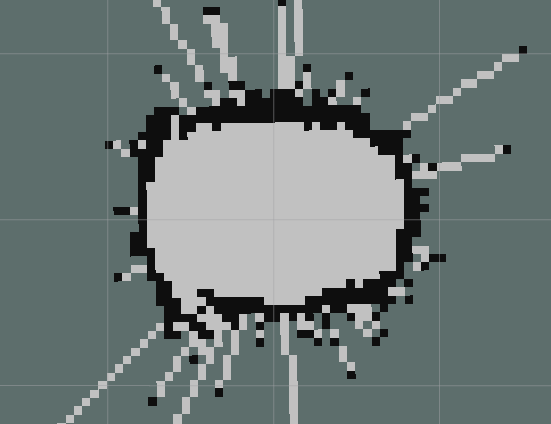
\includegraphics[width=\textwidth]{graphs/rectangle_map}
		\caption{With optimised parameters}
		\label{fig:gmapping_output/rect}
	\end{subfigure}

  \centering
  \begin{subfigure}[b]{0.4\textwidth}
    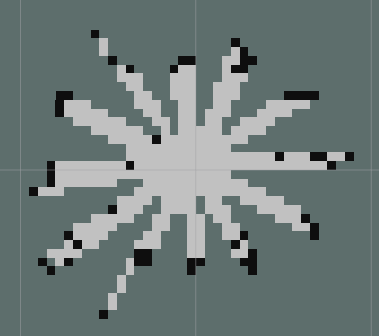
\includegraphics[width=\textwidth]{graphs/stripy_rect_map}
    \caption{Before optimising parameters}
    \label{fig:gmapping_output/stripy}
  \end{subfigure}
  ~
  \begin{subfigure}[b]{0.4\textwidth}
    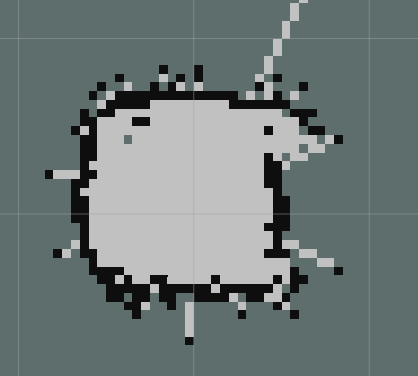
\includegraphics[width=\textwidth]{graphs/obstacle_map}
    \caption{Obstacle at right end of map}
    \label{fig:gmapping_output/obstacle}
  \end{subfigure}
  \caption{GMapping output}\label{fig:gmapping_output}
\end{figure}

Fixing all of this led to the generation of the map shown in Figure~\ref{fig:gmapping_output/stripy} when performed
on the largest rectangle that could be created in the maze. The robot was placed in the centre and made to rotate
slowly on the spot several times. This configuration was chosen to make the results easy to interpret.



This new map was far more accurate, with a correct scale and rough shape, but seemed to be missing many measurements
and not updating the map often. This was due again to the assumption of the use of LIDAR, which produces far too
much data to process exhaustively, so the mapping algorithm by default only updates the map with the last scan result
when the robot has moved 1 unit or rotated by 0.5 radians. This explains the 12 clear branches the map has formed,
as the map is only being updated 12 times. It is possible by a normally disabled parameter, \verb|temporalUpdate|,
to force the map to be updated at regular time. When this was set to the same rate as the ultrasonic scans were
being generated, the map shown in Figure~\ref{fig:gmapping_output/rect} was generated.

This output is clearly far better, and cursory examination showed the scale to be correct and accurate to within
\SI{1}{cm}. The rounded edges are to be expected, as the ultrasonics have a wide field of view, and therefore
reach the walls of corners before the points.

This experiment was repeated on another simple configuration, this time with a large square to the right of the
centre. This produced the map shown in Figure~\ref{fig:gmapping_output/obstacle}. This map is, as expected, somewhat less clean around the obstacle, but the obstacle is still clearly present. 

\section{Computer Vision}\label{soft/cv}
Computer vision is a cheap and effective way of gaining a high level
understanding of the environment (see Section~\ref{litreview/cv}). In this system, it was used to allow the robots to
identify other robots and objectives in the maze. Detecting other
robots was an essential component to allow communication between robots,
prevent robots mistakenly mapping other robots, and to recognise when
ultrasonic interference would occur.

\subsection{Design}\label{soft/cv/design}
The first detection system considered was a CNN, as discussed in Section
\ref{litreview/cv/objDet/CNN}. This is a very effective system which has
the advantage of
being able to classify instances of objects that it has not
seen before. This would be essential if the target objects of
the robot were not consistent, for instance if it was required to find
people in the search space. This was, however, not required
in the scope of this project. The major downside to this
system would be the time to implement. To construct a CNN for
this application would require the collection of a large data
set of images of the robots and goals, as well as the time
consuming process of tuning the CNN.

Feature-based object detection was also considered. As described in
Section \ref{litreview/cv/objDet/fb}, this only requires a picture to be
taken of the object and therefore takes far less time to
implement than the CNN solution. However, the accuracy and
consistency are largely dependent on the number of features
detected, and the algorithm's complexity grows relatively
quickly. The basic brute force algorithm involves comparing
every key point in the object image to every key point in the
frame image, which results in $\mathcal{O}(n^2)$ complexity. This can be streamlined, for instance, if it becomes impossible
for the distance to be low enough for a pair to be the best
match part way through the distance calculation, it does not
need to be finished~\cite{opencv_library}. The calculations for deciding the best
outline of the object also become more complicated, as there
is a lower true positive to false positive ratio as the
best matches (which are found first) are more likely to be
true positives. It was decided that this would be too
computationally intensive considering the strict constraint of
using an RPi.

The method used was by far the simplest considered. It identified the other robots and target
by their colour. This was only possible as each robot used had a distinct coloured chassis,
which lacks scalability, but was considered an acceptable simplification as this was not the
focus of the project.

This works by first converting the images from RGB to Hue-Saturation-Value (HSV) colour space,
simplifying the colour detection as the hue of the pixel is determined by a single value
instead of the ratio of three values. A colour can then be identified by a range of H values
and then minimum S and V values, which is far more intuitive than checking if it falls into a
range of ratios between R, G and B values.

\subsection{Implementation}\label{soft/cv/impl}
The \verb|vision_node| works using a ROS spin setup, with a \verb|spin()| function being
called at a set frequency until ROS closes.

A \verb|RobotDetector| object is declared which has the range of HSV values for each robot
and the goal, and also has a video capture object. It contains a \verb|search()| function which
takes a frame as a parameter and returns various details about each robot's presence in the
frame. \verb|search()| first calls \verb|get_colour_mask()| for each range of colour
values. This converts the image to HSV, then makes a frame, \verb|mask|, which is white where
the pixel is in range and and black when out of range. This is shown inListing
\ref{lst:get_colour_mask}. This also shows the handling of cases where the range of colours
crosses the zero point (as zero is adjacent to 255 in the hue value).

\begin{lstlisting}[caption={get\_colour\_mask in RobotDetector},label={lst:get_colour_mask} , language=python]

def get_colour_mask(self, frame, lower_hsv_bound, higher_hsv_bound):
    hsv_frame = cv2.cvtColor(frame, cv2.COLOR_BGR2HSV)

    if (lower_hsv_bound[0] > higher_hsv_bound[0]):
        mask1 = cv2.inRange(hsv_frame, np.array([0, lower_hsv_bound[1], lower_hsv_bound[2]]),
                            np.array(higher_hsv_bound))
        mask2 = cv2.inRange(hsv_frame, np.array(lower_hsv_bound),
                            np.array([179, higher_hsv_bound[1], higher_hsv_bound[2]]))
        mask = mask1 | mask2
    else:
        lower = np.array(lower_hsv_bound)
        upper = np.array(higher_hsv_bound)
        mask = cv2.inRange(hsv_frame, lower, upper)
\end{lstlisting}

The function then uses erosion and dilation functions provided by opencv to reduce noise in the
mask.

The contours in the mask are then iterated through to find the biggest, which is assumed to be
the object and the centre point and outline of the contour is found. If no contours are bigger
than a fixed size (measured in pixels) the object is assumed to not be in the image frame, and
the corresponding \verb|obj_found| variable is set to false. This process is shown in Listing~\ref{lst:cv_search_loop}.

\begin{lstlisting}[caption={Contour teration in \texttt{search()}}, label={lst:cv_search_loop}]
for c in contours:
    if cv2.contourArea(c) > max((300, maxsize)):
        maxsize = cv2.contourArea(c)
        cx, cy = self.get_centre_point(c)
        outline = self.get_outline(c)
        obj_found = True
\end{lstlisting}

These parameters are then returned to the \verb|_tick()| function which was called by
\verb|spin()|. This then renders debug information to the frame if it's performing a test, or
publishes the detected robot information via a ROS message consisting of a comma separated list of
objects detected in the last frame.

\subsection{Testing}\label{soft/cv/test}
Initial testing of the \verb|vision_node| was performed on a PC with a USB webcam. The
testing was performed by using the position information to render labelled rectangles to a real
time stream highlighting the position of the objects. The code for this is shown in Listing~\ref{lst:draw_rectangles}.

\begin{lstlisting}[caption={asd}, label={lst:draw_rectangles}]
for i, name in enumerate(names):
    if found[i]:
        #cv2.drawContours(frame, [outline], -1, (0, 255, 0), 2)
        #cv2.circle(frame, (cx, cy), 7, (255, 255, 255), -1)
        x, y, w, h = cv2.boundingRect(outlines[i])
        cv2.rectangle(frame, (x, y), (x + w, y + h), highlight_colours[i], 2)
        cv2.putText(frame, name, (x - 20, y - 20),
                    cv2.FONT_HERSHEY_SIMPLEX, 0.5, highlight_colours[i], 2)
\end{lstlisting}

\todo{caption??}

\noindent
An example of this running is shown in Figure~\ref{fig:cv_screenshot}.

\begin{figure}[!ht]
	\centering
	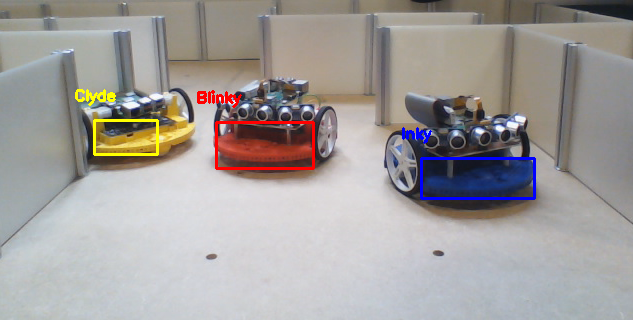
\includegraphics[width=1\textwidth]{ComputerVisionScreenshot.png}
	\caption{Computer vision PC test}\label{fig:cv_screenshot}
\end{figure}

The system was then tested on the RPi by monitoring the ROS topic \verb|robots_detected| to
test both the integration with the RPi and with ROS. Various detectable objects were moved in
and out of the frame and changes in the output were observed. This initially failed as the RPi
camera was connected using a CSI port, not a USB port, which OpenCV's VideoCapture function
does not support. When running on the RPi, this was replaced with imutil's VideoStream package.
Following this small change, the test performed as expected, consistently identifying which
objects were in frame.

Functionality was then added to record the feed to observe how the computer vision responded as
the robot was traversing the maze, however issues were encountered with frame rate, namely:
the functionality being too computationally intensive for the RPi in addition to all other
computation. This is therefore only used in debugging, and not usually active.

\section{Control Modules}\label{soft/control}

\todo[inline]{Path planning libraries}

Separate launch files were created for subsystems which rely on multiple nodes,
such as the communications system, so that they can be included in system launch
files along with any required parameters in a single line. The main launch file
used by every system-level launch is \verb|crues_control/robot.launch|, which
sets up all sensors and actuators, as well as nodes required for drive control,
sensor fusion, and SLAM. Launching a robot with a specific control node
merely requires creating a launch node which includes \verb|robot.launch| as
well as a single entry corresponding to the desired control node.
Listing~\ref{lst:control_launch_example} shows an example of a launch file for
a basic controller.

\begin{lstlisting}[caption={Launch file for null controller}, label={lst:control_launch_example}, style=xml]
<launch>
    <!--Empty controller used for debugging purposes.-->
    <include file="$(find crues_control)/launch/robot.launch" />
    <node name="null_controller" pkg="crues_control" type="roomba_control.py">
        <param name="turn_vel" type="double" value="0" />
        <param name="fwd_vel" type="double" value="0" />
        <param name="obstacle_range" type="double" value="0" />
        <remap from="~rate" to="encoder/rate" />
    </node>
</launch>
\end{lstlisting}


\subsection{Roomba Controller}\label{soft/control/roomba}

\todo[inline]{Two variations of Roomba. Present results here?}

\subsection{Debugging Controllers}\label{soft/control/debug}

\todo[inline]{Path controller, null controller, PID tuning controller}
